% --------------------------------------------------------------------------- %
% Author:          Joey Dumont                <joey.dumont@gmail.com>         %
% Date created:    Jun 19th, 2015                                             %
% Date modified:   Jun 19th, 2015                                             %
% Description:     Prepared for IHPCSS 2015.                                  %
%                  TikZ code to show the DomainDecomposition method.          %
% License:         CC0                                                        %
%                  <https://creativecommons.org/publicdomain/zero/1.0>        %
% --------------------------------------------------------------------------- %

\documentclass[tikz]{standalone}
\usepackage[charted]{mathdesign}
\usepackage{fontspec}
\setmainfont{Oswald}

\usetikzlibrary{calc}

\newcommand{\focal}{5}
\newcommand{\parabola}[1]{\pgfmathsetmacro{\myvalue}{#1*#1/(4*\focal)-\focal}}
\newcommand{\iparabola}[1]{\pgfmathsetmacro{\myivalue}{sqrt(4*\focal*(#1+\focal))}}
\begin{document}

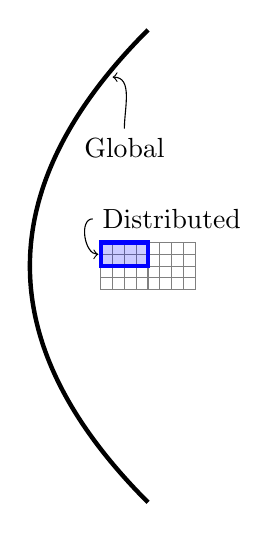
\begin{tikzpicture}[scale=0.3]
  \draw[domain=-\focal:0,samples=1000,ultra thick] plot (\x,{sqrt(4*\focal*(\x+\focal))});
  \draw[domain=-\focal:0,samples=1000,ultra thick] plot (\x,{-sqrt(4*\focal*(\x+\focal))});

  \draw[step=0.5,gray,thin] (-2,-1) grid  (2,1);
  \draw[ultra thick,blue,fill=blue,fill opacity=0.2](-2,0) node[coordinate,anchor=east] (dist) {} rectangle (0,1) ;

  \node (global) at (-1,5) {Global};
  \node (distText) at (1,2)  {Distributed};

  \draw (distText) edge[out=180,in=180,->] ($(dist.east)+(-0.1,0.5)$);
  \draw (global)   edge[out=90,in=0,->] (-1.5,8);


\end{tikzpicture}

\end{document}
